% Created 2021-03-25 jeu. 12:02
% Intended LaTeX compiler: pdflatex
\documentclass[a4paper,12pt]{article}
\usepackage[position=top,labelformat=empty]{subfig}
\usepackage{caption}
\usepackage[hmargin=2cm,vmargin=3cm]{geometry}


\usepackage{amsmath}
\usepackage{caption,graphicx,subcaption}
\usepackage[boxed]{algorithm2e}
\date{\today}
\title{A Mirror encoding combined with the FFT for a fast heuristic of the RNA folding dynamics}
\begin{document}

\maketitle

\section{Abstract}
\label{sec:org9d90e07}
\begin{itemize}
\item Simple and fast heuristic for the folding path of RNAs.
\item It is straightforward to model Pseudoknots
\item It's performance is comparable to exact method on the RNA folding problem
\item It follows a simple idea which naively corresponds to RNA folds mechanism
(many BPs formed at once to compensate for the lost of entropy)
\item Among the 50 predicted structures, in average, at least one has pvv \textasciitilde{} 74\% and
sensitivity \textasciitilde{} 76\%.
\item We propose a fast algorithm method based on the FFT to search for high density
BP regions.
\end{itemize}

\clearpage
\section{Introduction}
\label{sec:orgb808b13}
\subsection{RNA folding dynamics}
\label{sec:orga1ee2ce}
bla bla dynamic of secondary structure relevant bla biological function.

\subsection{RNA folding dynamics}
\label{sec:orga0d38a2}
\begin{enumerate}
\item Description of RNA structure
\item going up to the 2ndary structure only
\item Simple rules to compute a structure: multiple BPs compensate the lost of
entropy during the folding process.
\end{enumerate}

\subsection{Existing methods}
\label{sec:org829134c}
\begin{enumerate}
\item MC sampling: kinefold; atomic moves; MC-style simulation
\item Barrier trees from conformation landscape subopt tree: Sample from the
boltzmann ensemble of structures
\end{enumerate}

\clearpage
\section{FFT based folding dynamic heuristic}
\label{sec:org2c0a75f}
\begin{enumerate}
\item Encoding into two complementary strands
\item Search for high BPs regions
\item Use a sliding window to form large consecutive BPs
\item split the strands into interior and exterior
\item start again from 2) for the two sub-sequences
\end{enumerate}

We now describe the heuristic folding algorithm starting from one sequence S and
its associated unfolded structure of lenght L. We first create a numerical
representation of S where each type of nucleotide in replaced by a unit vector
of 4 components:
\begin{equation}
\begin{split}
A \rightarrow \begin{pmatrix} 1 0 0 0 \end{pmatrix}
U \rightarrow \begin{pmatrix} 0 0 0 1 \end{pmatrix}
C \rightarrow \begin{pmatrix} 0 1 0 0 \end{pmatrix}
G \rightarrow \begin{pmatrix} 0 0 1 0 \end{pmatrix}
\end{split}
\end{equation}
which gives us a \(4 \times L\) matrix we call X where each row is a nucleotide
type channel. Here, the first row would be the A channel which we refer to as
\(X^A\). Then, we create a second copy for which we revert the order of the
sequence and use the following complementary encoding:
\begin{equation}
\begin{split}
\bar{A} \rightarrow \begin{pmatrix} 0 0 0 w_{\scalebox{0.5}{AU}} \end{pmatrix}
\bar{U} \rightarrow \begin{pmatrix} w_{\scalebox{0.5}{AU}} w_{\scalebox{0.5}{GU}} 0 0 \end{pmatrix}
\bar{C} \rightarrow \begin{pmatrix} 0 0 w_{\scalebox{0.5}{GC}} 0 \end{pmatrix}
\bar{G} \rightarrow \begin{pmatrix} 0 w_{\scalebox{0.5}{GC}} 0 w_{\scalebox{0.5}{GU}} \end{pmatrix}
\end{split}
\end{equation}
where \(w_{AU}\), \(w_{GC}\), \(w_{GU\) are tunable parameters for the next step. We
call this new copy \bar{X}, the mirror of X.

For each of the 4 components, we compute the correlation between X and \bar{X}
and simply sum up the four channels to obtain the correlation between the two
copies:
\begin{equation}
cor(k) = (c_{X^A,\bar{X}^A}(k) + c_{X^U,\bar{X}^U}(k) + c_{X^G,\bar{X}^G}(k) + c_{X^C,\bar{X}^C}(k)) / min(k, 2 \times L-k)
\end{equation}
where \(c_{X^A,\bar{X}^A(k)\) is the correlation in the \(A\) channel between the
two copies. The correlation \(cor(k)\) gives the average number of base pairs for
a positional lag \(k\). One channel correlation between the copies is given by:
\begin{equation}
c_{X^A,\bar{X}^A}(k) = \sum\limits_{1\leq i \leq L, 1 \leq i + k \leq M} X^A(i) \times \bar{X}^A(i+k)
\end{equation}
where \(X^A(i)\) and \(\bar{X}^A(i+k)\) are the A channel of site \(i\) and \(i+k\).
X\textsuperscript{A}(i) \texttimes{} \bar{X}\textsuperscript{A}(i+k) is non zero if sites \(i\) and \(i+k\) can form a base
pair, and will be the value of the chosen weight as described above. Although
this operation requires \(O(N^2)\) operation, it can take advantage of the FFT
which reduces drastically its complexity to \(O(Nlog(N))\).

The large correlation values between the two copies indicates the positional lag
between at which the base pair density is high. Therefore, we use a sliding
window strategy to search for the longest consecutive base pairs within the
positional lag. Since the copies are symmetrical, we only need to slide over one
half of the positional lag. Once the longest base pairs are identified, we
simply compute the free energy change when those base pair are formed. We
perform the same search for the \(n\) highest correlation lags, which gives us \(n\)
possible possibilities. Then, we added to the current structure the base pairs
that gives the best change of energy.

We are now left with two segments, the interior and exterior of the group of
consecutive base pairs formed. The two exterior fragments are concatenated
together. Then, we simply apply recursively the same procedure on the two
segments separately in a "Breath First" fashion to form new consecutive base
pairs, until no base pair formation can improve the energy. However, it is
straightforward to consider pseudoknots by simply concatenating all the
fragments left.

The algorithm described so far tends to be stuck in the first local minima found
along the folding trajectory. To alleviate this, we propose a stacking procedure
where the 50 best trajectories are stored in a stack and evolved in parallel.
Hence, it offers the flexibility of overcoming some energy barriers. \textbf{Figure}
shows the whole procedure.

\clearpage
\section{Folding RNAs}
\label{sec:org0c55b0f}
\begin{enumerate}
\item comparisons to DP folding algorithm -> RNAfold and MFE prediction or MEA
\item Comparisons to ML folding algorithm -> Mxfold or Contextfold
\item The discrepancy between FFT and RNAfold for the folding task can be explained
by the greedyness of the algorithm.
\item Show the best trajectory among the 50 predicted and its PVV performance =>
means that one trajectory is relevant most of the case. Could be combine with
ML method to determine which one.
\item How natural loop compositions are distributed -> bias toward some specific
composition while.
\item Show two folding trajectories, one where it works, and one where the
greedyness is a problem.
\end{enumerate}

To evaluate the relevance of the folding trajectories produced, we benchmarked
the algorithm performance for the folding task. In addition, we want to assess
the effect of sequence length on these predictions.

We compared the performance of the MFE structure computed by RNAfold and the
performance of a machine learning approach implemented in Contrafold/Mxfold.

The performance analysis were performed sequence-length-wise to asses the impact
of length increase.

To investigate the region of the structure space where the thermodynamic model
tends to fail, we computed the composition content of the natural structures and
mapped the ones that had a low PVV score. It shows that the MFE tends to fail
when the structure contains a high proportion of interior loops as shown in
\textbf{figure}.

\begin{figure}[htbp]
\centering
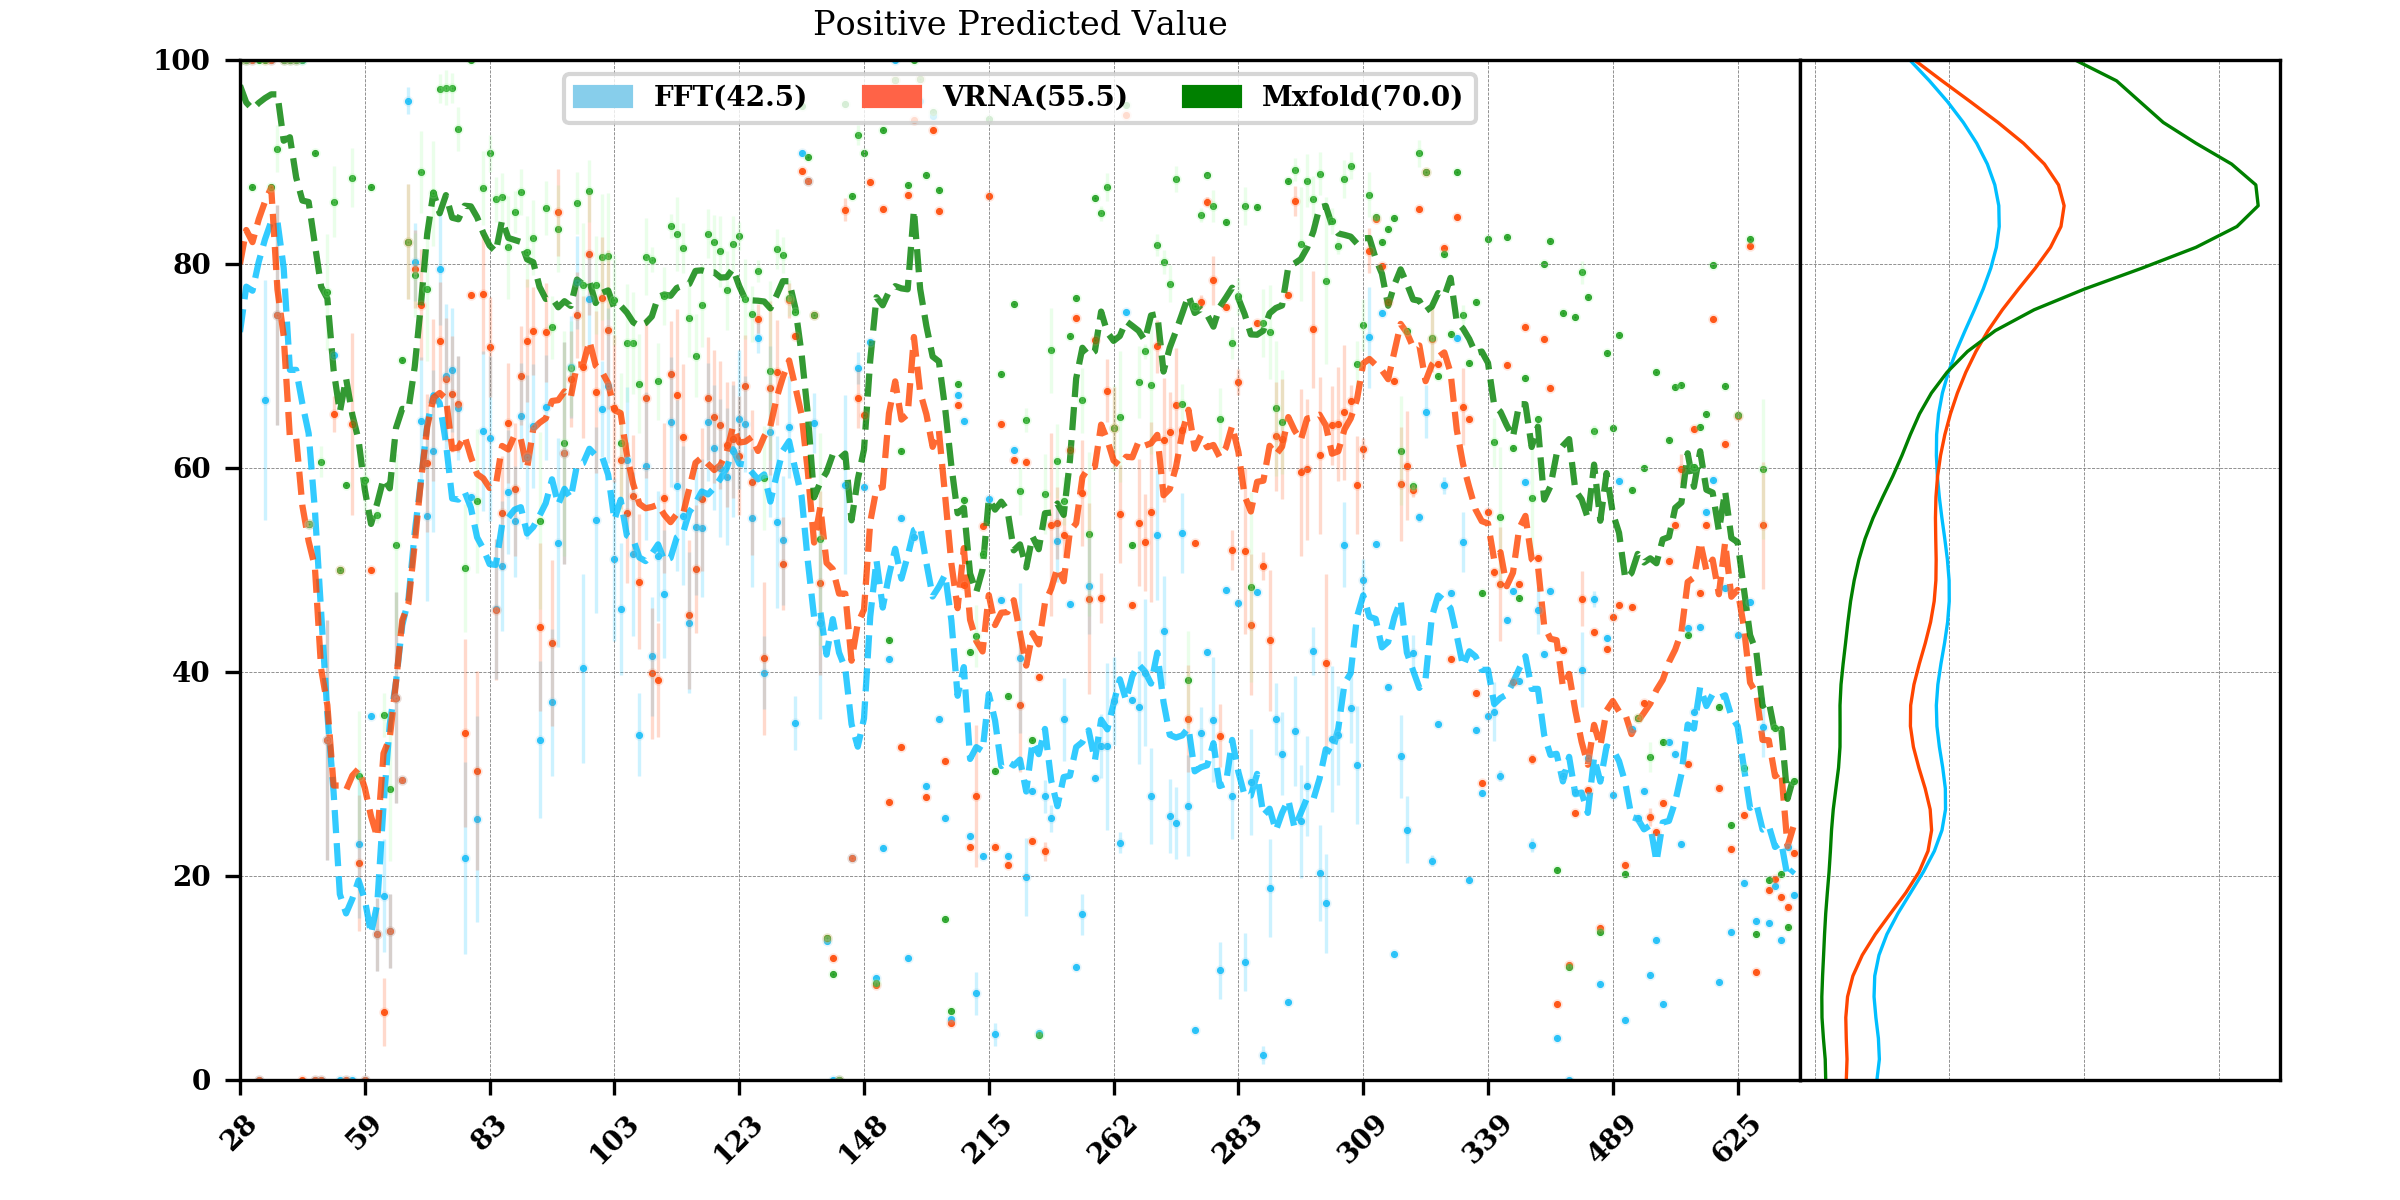
\includegraphics[width=.9\linewidth]{img/comp_100n_30s_pvv.png}
\caption{Folding comparison by taking the best energy among the 30 predicted trajectories}
\end{figure}

\begin{figure}[htbp]
\centering
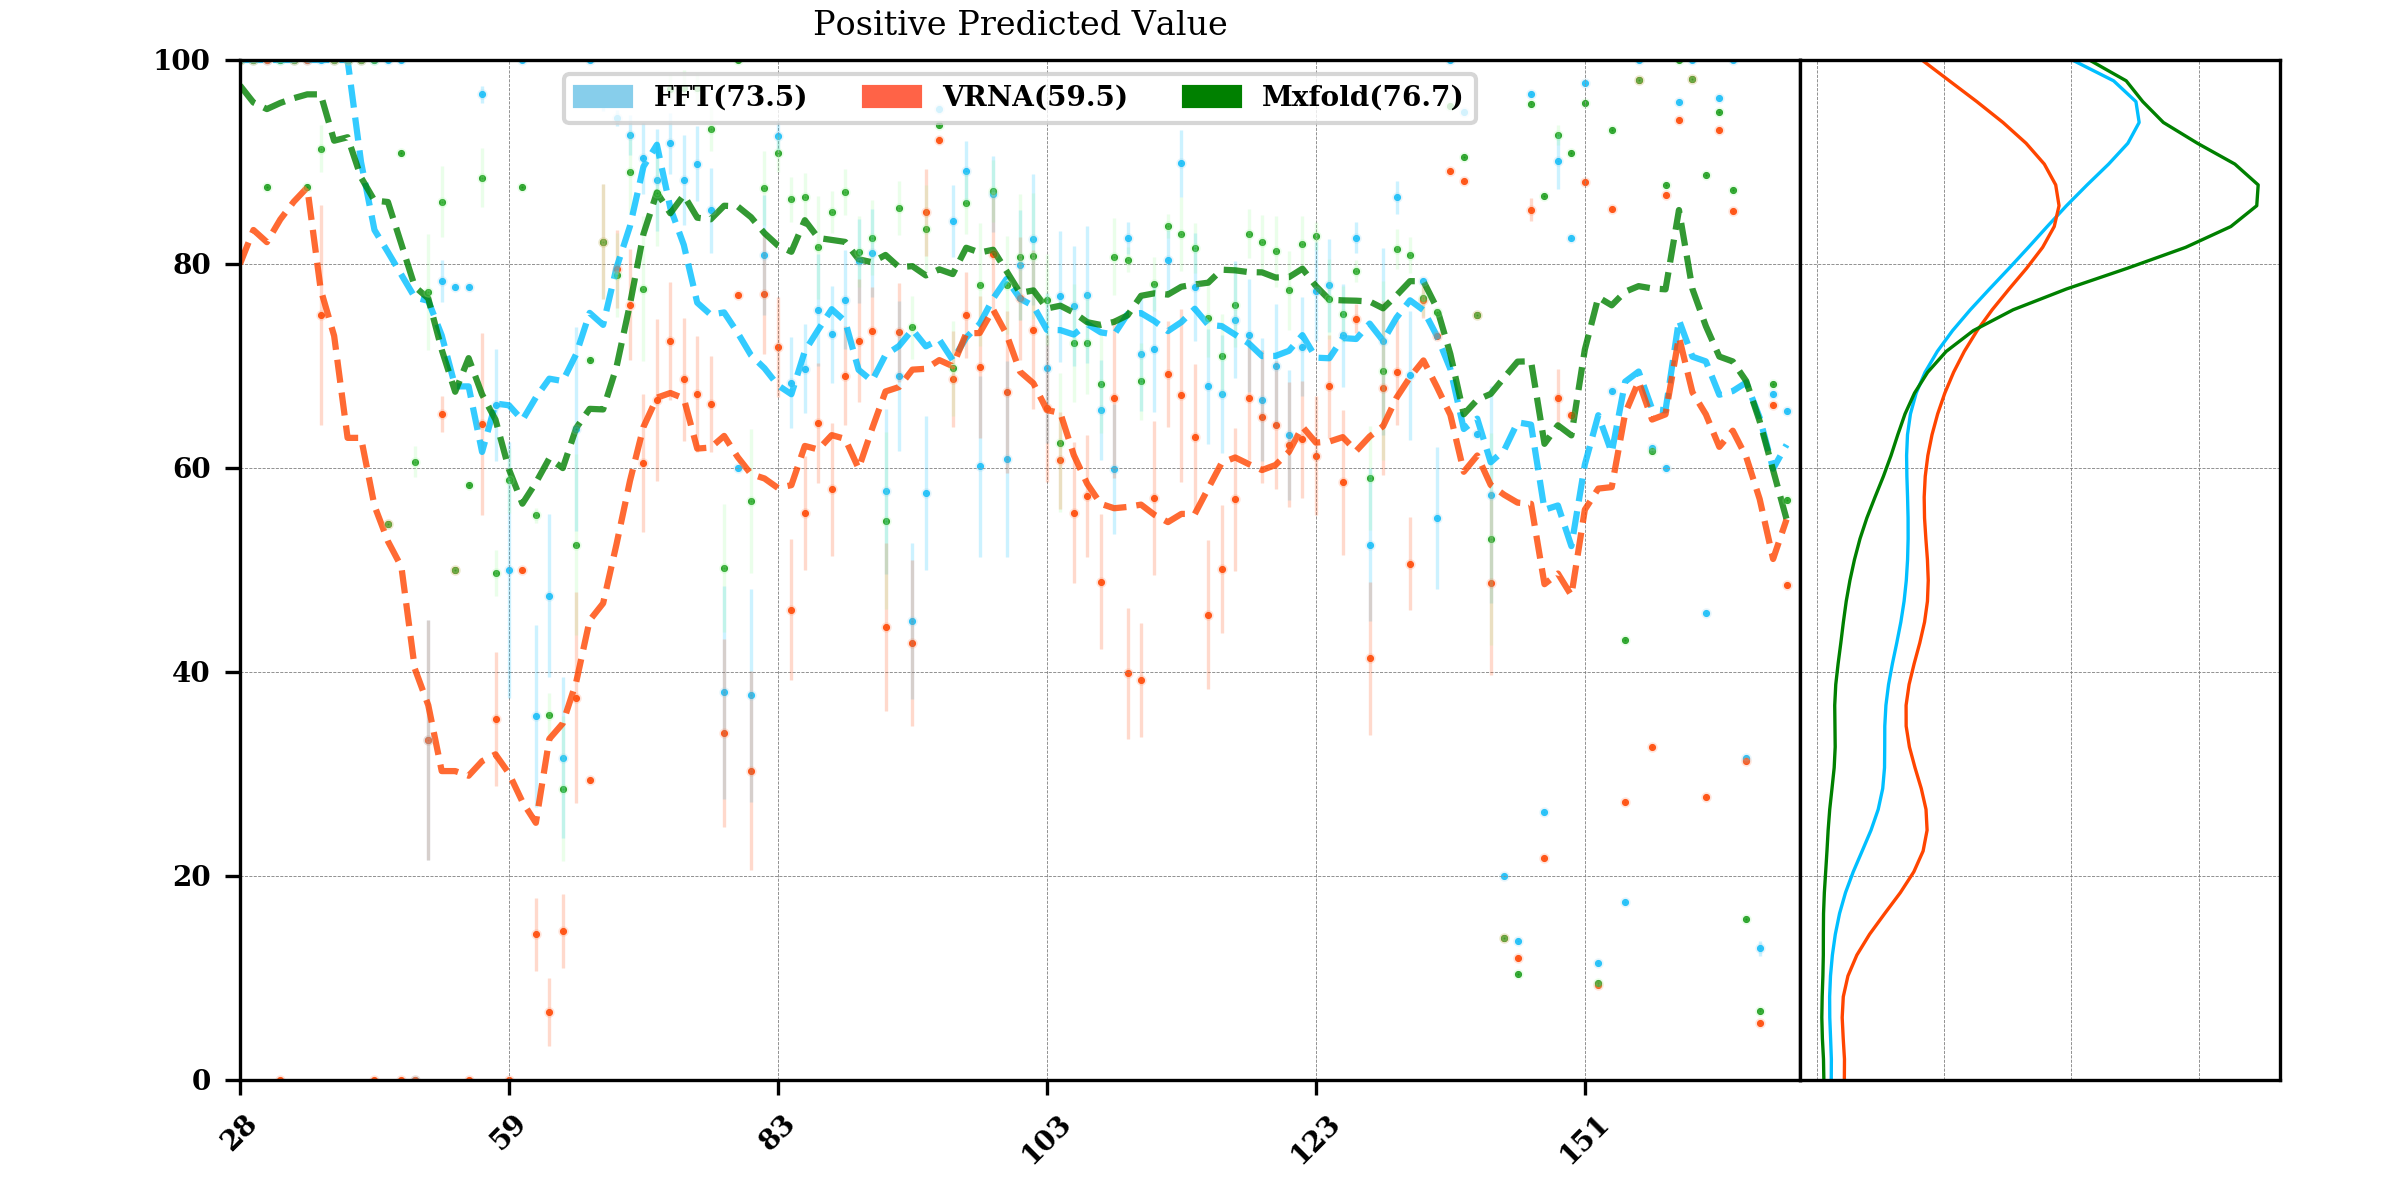
\includegraphics[width=.9\linewidth]{img/comp_max_50n_50_stacks.png}
\caption{Is there a good trajectory among 50 saved trajectories}
\end{figure}

\begin{figure}[htbp]
\centering
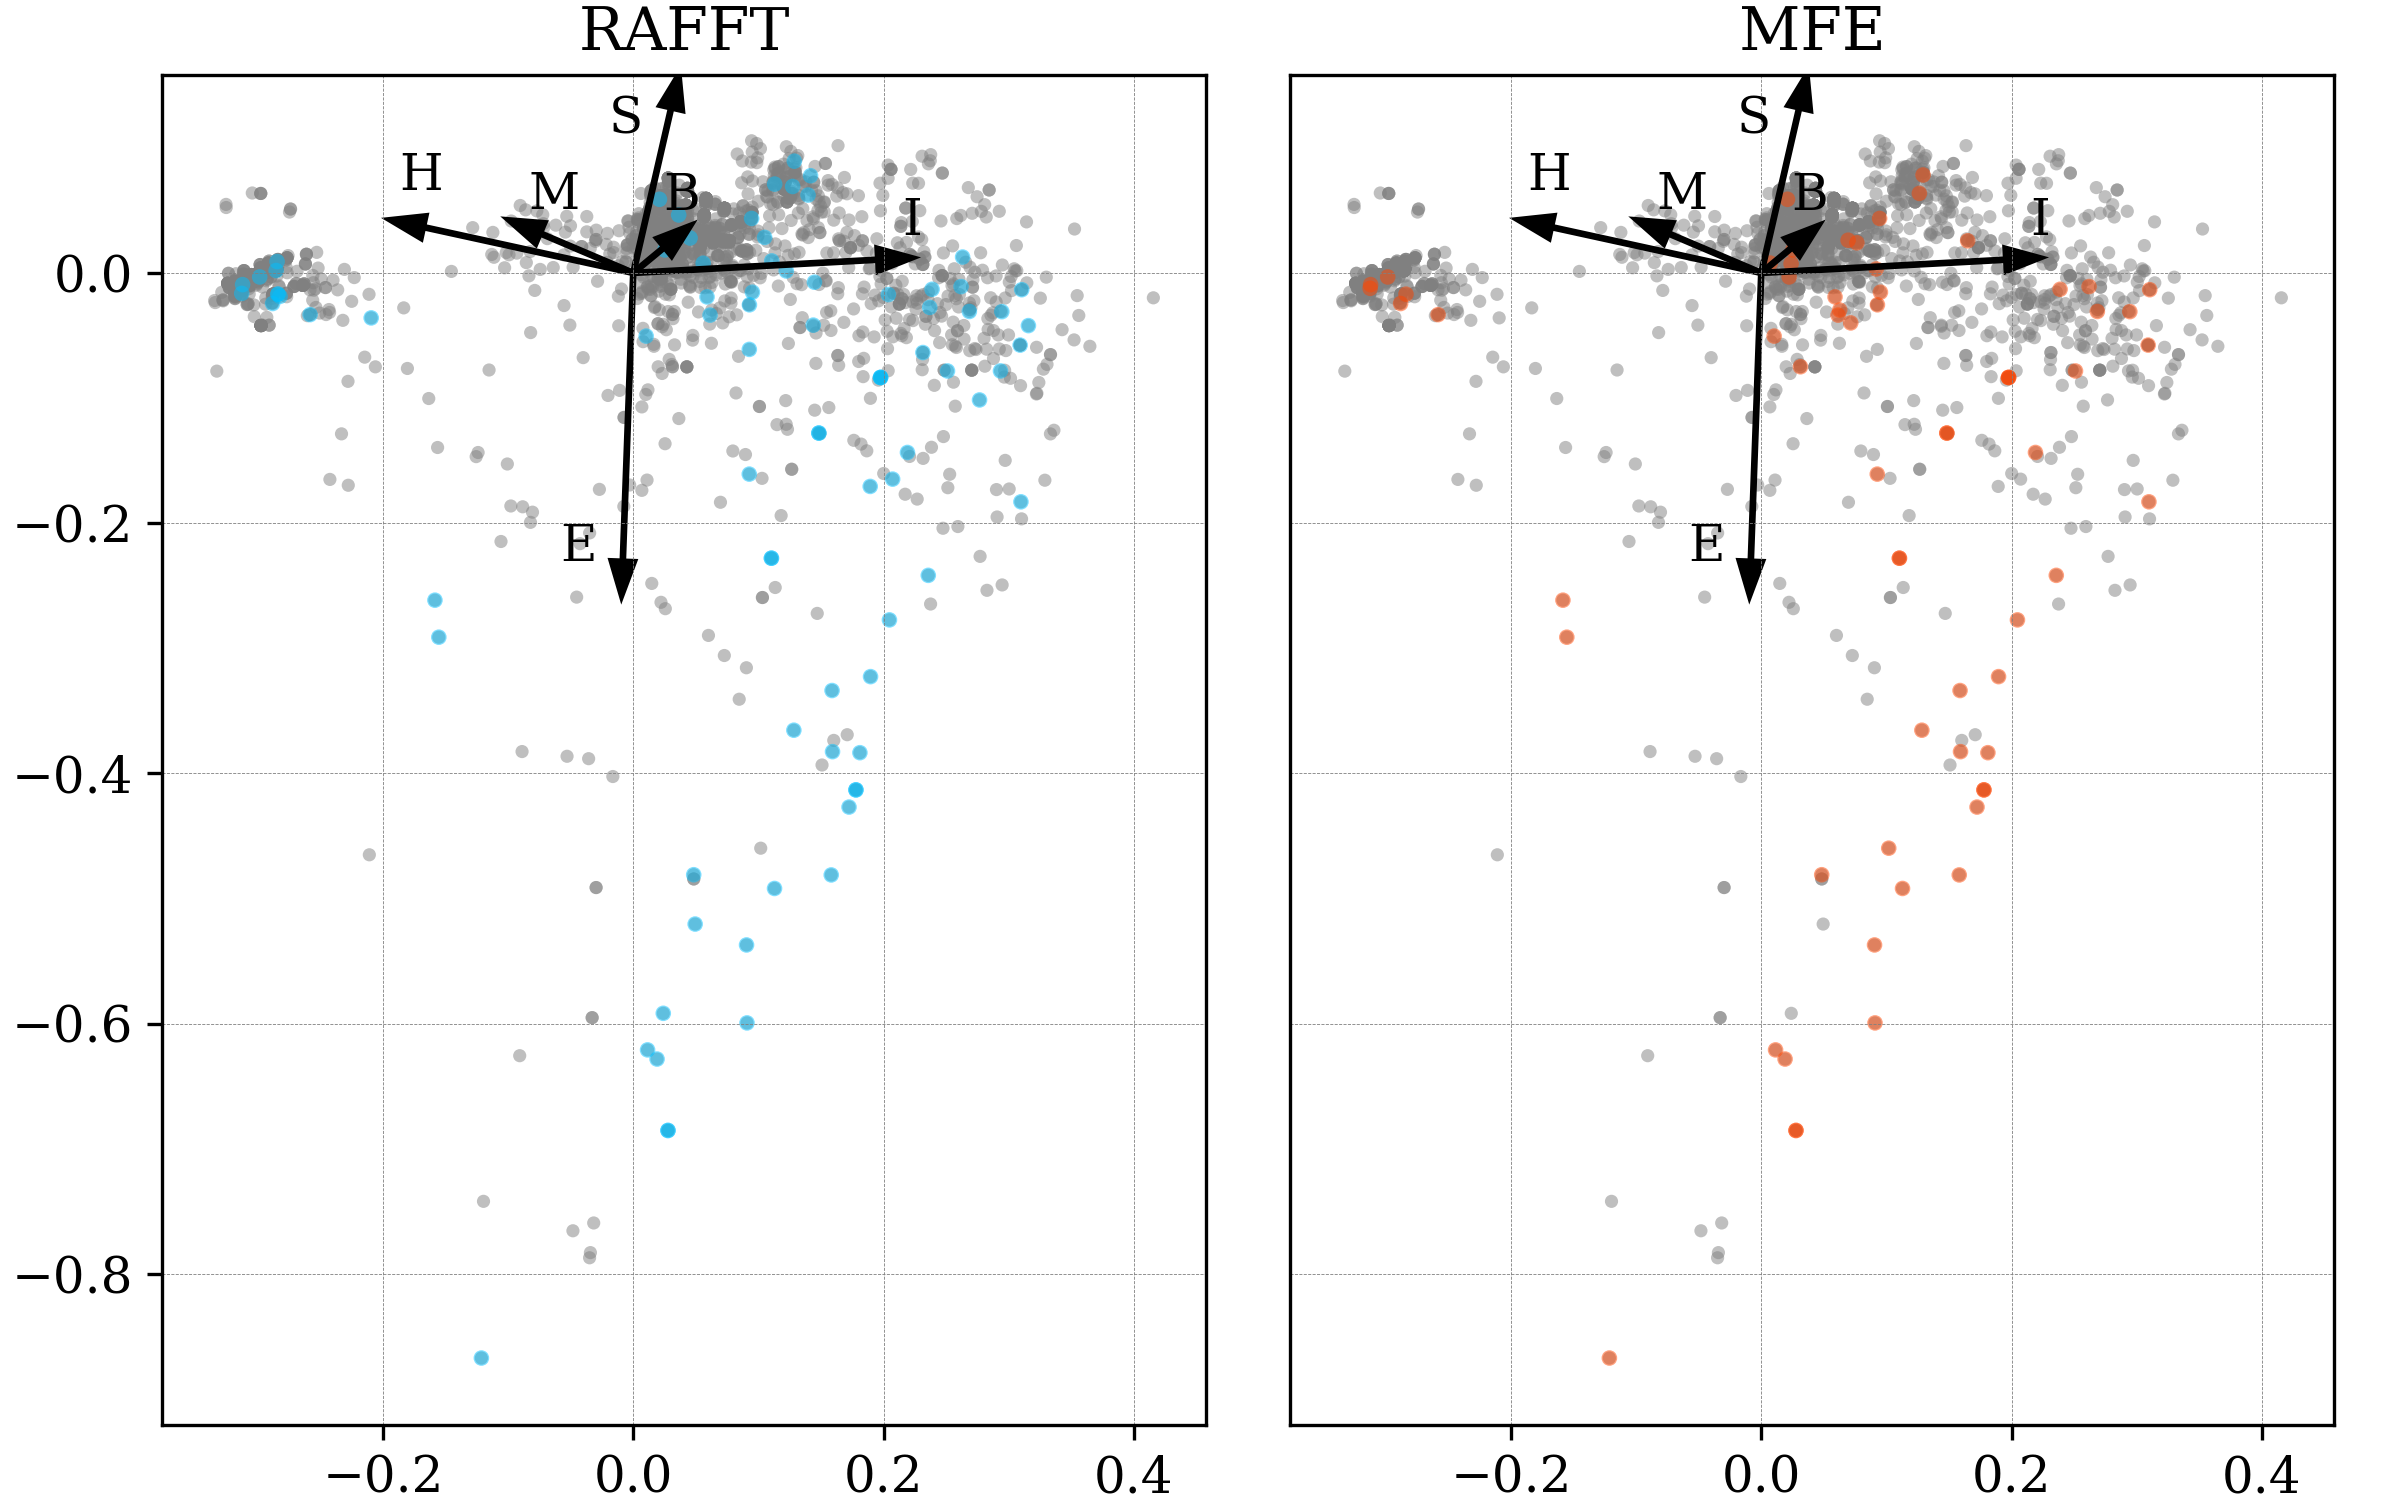
\includegraphics[width=.9\linewidth]{img/comp_fails.png}
\caption{where does the methods failed? PCA RNAfold, Mxfold, FFT, and}
\end{figure}

\section{Methods}
\label{sec:org306b1fe}
\begin{enumerate}
\item Dataset used
\begin{enumerate}
\item We considered all structures with nrj < 0 and no pseudoknot (since the
energy parameters doesn't take them into account).
\item We studied a smaller subsets of shorter sequences length <= 200 nuc in
which we expect the thermodynamic model to be the most accurate. (maybe
put that above)
\end{enumerate}
\item Folding parameter applied for all methods considered
\item Analysis: PVV and sensitivity + PCA and composition extraction
\end{enumerate}
\subsection{Datasets}
\label{sec:org4ee8a03}
We formed two sub-datasets based on the ArchiveII (\textbf{ref}) dataset. We first
removed from all the structure containing pseudoknot since all tool considered
here don't handle pseudoknots. Next, we removed all the structures which were
evaluated with a positive energy or null energy with the Turner 2004 energy
parameters. Since positive energies means that the completely unfolded structure
is more stable than the native one, we assume that those structure are not well
modeled by the parameter set.

\clearpage
\section{Concluding discussion}
\label{sec:org861e6ca}
\subsection{Good stuff}
\label{sec:orge4ec0ab}
\begin{enumerate}
\item Simple heuristic to compute folding path
\item Versatile method: allow simple modeling of pseudoknot and more information
can be encoded in the mirror representation.
\item Performance is comparable although not as good as state of the art in the
folding task.
\item One trajectory among the selected produce good structures (close with better
accuracy than ML methods).
\end{enumerate}

\subsection{limits}
\label{sec:org61e50bb}
\begin{enumerate}
\item Choosing the maximum number each time is not an optimal choice
\item In average, the scores are not good. Only a few out of the predicted
structures have good scores.
\item The quality of the prediction degrade drastically when the size > 250 from
74\% -> 50\%.
\begin{enumerate}
\item The stacking method might one cause however, since MFE is degraded as
well, we believe that it might partly explain by the thermodynamic model
accuracy.
\end{enumerate}
\item The distribution of loop types composition seems to differ between the
Boltzmann ensemble and the natural structures.
\end{enumerate}
\end{document}
